\documentclass[11pt]{article}

\usepackage{cite}
\usepackage{graphicx}
\usepackage{wrapfig}
\usepackage{listings}
\usepackage{hyperref}
\usepackage{titlesec}
\usepackage{url}
\usepackage{float}
\usepackage{caption}
\usepackage{subcaption}

% Margins
% \topmargin=-0.45in
% \evensidemargin=0in
% \oddsidemargin=0in
% \textwidth=6.5in
% \textheight=9.0in
% \headsep=0.25in

\setcounter{secnumdepth}{4}

\titleformat{\paragraph}
{\normalfont\normalsize\bfseries}{\theparagraph}{1em}{}
\titlespacing*{\paragraph}
{0pt}{3.25ex plus 1ex minus .2ex}{1.5ex plus .2ex}

\lstdefinestyle{myListingStyle} 
{
	basicstyle = \small\ttfamily,
    breaklines = true,
}
\title{ My Little Operating System }
\author{ Sam da Costa }
\date{\today \endgraf \bigskip Project Supervisor: Jim Garside}

\begin{document}
\maketitle	
\pagebreak


\tableofcontents
\pagebreak

%--Paper--

\section{Introduction}
Operating Systems\cite{os} are used everywhere in the modern day. Nowadays, even when performing trivial actions like ordering take-out food or checking out at a supermarket, people engage with an operating system. These systems are so ubiquitous that people outside of the field of computer science may not even realise that they are interacting with one. If you were  to ask these people what an operating system was, they would probably give you an answer like, Windows \cite{windows}, MacOS \cite{apple} or Linux \cite{linux}. In reality the definition of an Operating System extends further beyond the bounds of OS's for personal computers. At its core an Operating System is the low-level software which supports the basic functions of a computer, tasks such as scheduling and controlling IO devices. Understanding the role Operating System's play for modern computers should be important for high level programmers as the code they write will always be subject to the Operating System's management of the computer. ARM provides a good platform for understanding Operating Systems as it allows an experience of a system before any software is present. This completely `clean slate` to build on can build a programmers understanding of an Operating System as before any application code can be written, the programmer has to tackle at least some of the problems. 

\subsection{Project Goals}
At the start of the project I derived three main goals.
\subsubsection{Objective 1}
\label{obj1}
% Support basic functions
The first goal was to support the basic function of a computer. This includes providing an environment for user code to be run in and the tools required for a user access privileged components of the system. This includes: providing an Supervisor Call Handler (SVC) to service calls such as calls to graphical output, providing a reset handler to reset relevant parts of the memory to a workable state and providing access to input and output devices. 
\subsubsection{Objective 2}
\label{obj2}
% Handle realistic Input
The second goal was to design, develop and interface a virtual keyboard with the system. This keyboard should at a minimum provide the ability to convey keystrokes to the system. A more sophisticated implementation would be able to recognise combinations of keystrokes and report the use of control keys being pressed to move the cursor. I propose to use a virtual keyboard as I intend the emulate an ARM processor rather than develop on a real one. 
\subsubsection{Objective 3}
\label{obj3}
% Develop a Process Management System
The third goal was the development and implementation of a thread management system for my processor. This differs slightly from the implementation of process management \cite{process} on modern operating systems as my thread management system will operate in a single memory space. Typical process management systems operate in separate virtual memory spaces. While it may be possible to implement this on an arm chip, the lack of hardware support on the particular chip I have would make this a hard task to accomplish with only software. Therefore, I opt to develop threads rather than processes. In addition to this management system, I also need to develop the required methods to give the user access to use the management system as a tool. These methods include the ability to create and end threads. Further implementations could include the ability to enable smooth communications between threads. 
\pagebreak
\section{Motivation and Background}
\label{motivations}
\subsection{Motivations}
The motivation for this project stems from previous courses I have taken such as `Fundamentals of Computer Architecture', `Microcontrollers' and `Operating Systems'. When taking these course I really enjoyed the challenges behind working within an ARM based environment, such as working with few `variables' and having no pre-made software available to you. For me, these challenges raised the question of how viable it is to write an operating system for a microcontroller.
While I had done a simple form of this for my Microcontrollers course, I wanted to take it further by implementing more complex features. In addition to this I wanted to improve upon the work I had done. This work had been relatively rushed and messy as I was having to learn on the go, and I did not have much time to re-factor. From this I derived two main goals for this project; I wanted to develop an OS which was better structured, and I wanted to develop some sort of process management service for the ARM chip. The operating systems course should help with the development of the process management service, as the notes I have explain how operating systems manage processes and threads within an OS. This project is more concerned with developing threads rather than processes, the distinction being that a thread is usually a segment of a program running as a process. 

Finding ways of keeping my work organised became a large part of this project for me. Most of my programming experience has, until now, been focused on higher level languages such as C\# and Java. Due to this, developing for a low level language felt quite jarring due to the following characteristics of ARM, program structure can become disorganised and hard to read without self-imposed discipline. Braces and indentation are not enforced, which would usually expose the control flow of the program. Automated type checking does not exist. These problems reinforced the necessity of commenting in all my code, even beyond ARM. Consistently commenting an a specific style also became a key strategy to ensuring my code was readable. I often found myself trading off legibility against efficiency.

\subsection{Background}
The system I built has it roots in the Microcontroller's course, and it derives much of its environment from the work done there. The system was built for the graphical debugger named `Komodo' \cite{kmd}. This acts as a `front end' for `back end' processor models. In my case the model I used was  and emulator called `Jimulator'. It also provides me with the assembler for my ARM code, as well as the ability to load and run the assembled code on a virtual ARM processor. The debugging facilities it provides allow me to pause the code at breakpoints I set and inspect the state of the processor's memory and registers. My working environment also consists of a few plug-ins for Jimulator. These plug-ins are as follows:

\begin{itemize}
	\item An 8-bit clock-based timer exposed as a byte in memory.
	\item 3 x 4 virtual keypad with an interface set-up in the memory.
	\item A 320px x 240px virtual RGB display with an interface set-up in the memory of the ARM chip.
\end{itemize}

These plug-ins for the Jimulator emulator expose themselves at static memory addresses with various interfaces.
The timer appears as a read-only memory location at 0xF100\_1010. This timer is free-running and increments at 1kHz. 
The keypad simulates a matrix keypad. It works by allowing the ARM processor to activate scan lines and read the resulting input to determine which keys have been pressed. It also appears as a single byte containing both the scan-line bits and the resulting output bits.

\begin{figure}[ht!]
	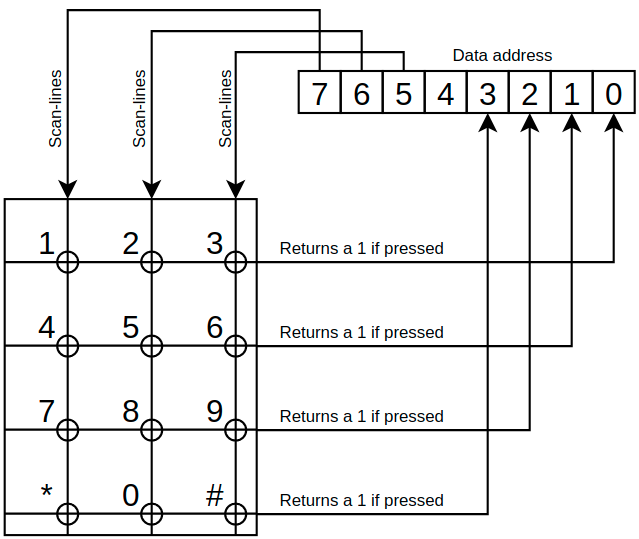
\includegraphics[width=0.5\linewidth]{figures/keypad.png}\centering
	\caption{Keypad Matrix Setup}
	\label{fig:keypad}
\end{figure}

The virtual screen is made of a `vscreen' program, connected to the Jimulator via a plug-in. The plug-in exposes the access to the screen via a frame buffer set-up in memory starting at 0xAC00\_0000. The memory set-up consists of 3 bytes for each pixel running left to right, top to bottom. The 3 bytes represent the RGB values of the corresponding pixel.

\begin{figure}[ht!]
	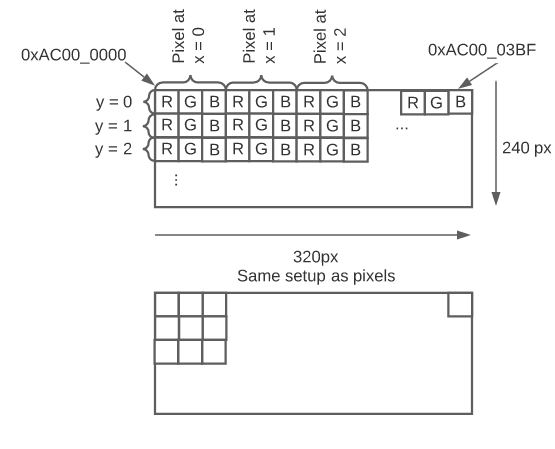
\includegraphics[width=\linewidth]{figures/LCD.png}\centering
	\caption{Frame buffer memory set-up}
	\label{fig:LCDMem}
\end{figure}

The system I created required me to modify this starting environment by replacing the keypad with an new plug-in, which created and handled a new virtual keyboard as detailed later in \autoref{chap:virtualKeyboard}. 

\pagebreak
\section{The Virtual Keyboard}
\subsection{The development environment}
The virtual keyboard took far more time than I had initially anticipated. It required me to delve into the installation process for Komodo as I had no knowledge of how to attach software to Komodo. When browsing through the set-up folder and bash script for Komodo, I found the Jimulator plug-ins which my tutor had pointed me in the direction of. These plug-ins act as event handlers for the ARM chip. They can respond to things like SVC commands, memory reads and memory writes. The useful thing about these plugins is that they can also affect the chip in various ways by causing interrupt signals and writing data to specific registers. This is essentially how all the input and output was handled in COMP151111. In this course the students would make an SVC\_0 call which Jimulator would intercept, and then output R0 to the built-in terminal. In much the same way a call to SVC\_1 would be intercepted by Jimulator causing a read from the terminal into R0. The scripts included in the default installation of Komodo also included a virtual keypad, a timer, and a virtual screen. I had used the screen and keypad before, but I wanted more keys for the keypad, in order to make inputting letters easier. Naturally, the keypad plug-in became my reference for creating a plug-in as it was the closest in purpose for what I wanted to achieve. 

I determined from the keypad plug-in that the actual interface seen by the user was a simple python script executed during Komodo's start-up. This script parsed an XML file which defined the layout of the keypad. This script then also passed the states of the buttons to a piece of shared memory. The shared memory was then attached in the plug-in script and when ever a read was made to the keypads' location, the plug-in would intercept it and update it according to the contents of the shared memory. The last bit of knowledge I needed was how to compile the plug-in, into something jimulator could actually work with. From reading the make file I determined that the code had to bed compiled with the --shared flag to compile a shared object and the \verb|fPIC| flag to indicate it is a library and may be executed from anywhere so that its jumps need to be calculated relatively rather than absolutely.
\subsection{Design}
\subsubsection{Virtual Keyboard Hardware Interfaces}
The virtual keyboard design is very similar in concept to the virtual keypad explained above. However, it differs hugely in how it appears as a peripheral in the ARM environment. The keypad used in the COMP22712 labs appears as a single byte, in which bits 7-5 are set in turn to allow bits 3 - 0 to be scanned into. This set-up requires the system to scan they keyboard themselves and denounce the result. While this is also a possible protocol to implement with the larger keyboard I built, I felt it made more sense to have the virtual keyboard appear as 3 bytes, one to trigger the data change, one to represent an ASCII character, one to represent the direction of the button interaction (pushed or unpushed).

The advantages of handling the keyboard this way are that I don't have to have as much processing on the ARM side. This is very helpful as the code required to scan a virtual keyboard can be quite cumbersome and time-consuming. This interface also allows me to mimic modern hardware, which would send ASCII codes, rather than requiring the processor to manage the IO more manually. 
\subsubsection{Keyboard Design}
I used the python library glade to model the keyboard. Unfortunately, lots of these buttons are there for appearance's sake only, as this keyboard does not implement a full ASCII character set. I chose to do this as I felt the time to benefit ratio did not warrant spending more time on this. While I could have implemented more control characters, I would be highly unlikely to use them so, I felt it would be wasted time. 

\begin{figure}[ht!]
	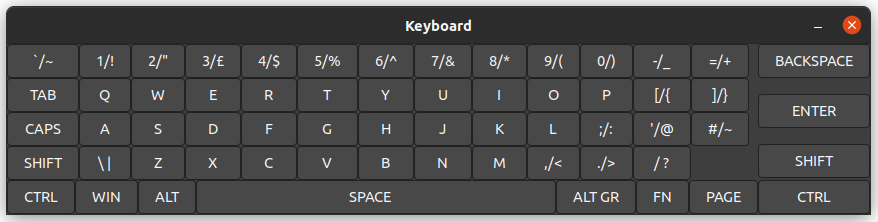
\includegraphics[width=\linewidth]{figures/keyboard.png}
	\caption{The final design of the virtual keyboard.}
	\label{fig:keyboard}
\end{figure} 
 
I managed to implement working characters from ASCII 0x20 to 0x7F as well as working caps-lock, shift, backspace, enter and tab characters. 



\subsection{Implementation}
The initial protocol I developed to handle input is as follows.

\begin{itemize}
	\item The user presses a button on the keyboard
	\item Glade signals the plug-in that a key has been pressed (or unpressed) via the shared memory
	\item The plug-in reads the data and make it ready to write.
	\item The plug-in throws an interrupt.
	\item The interrupt routine receives the interrupt and writes a 1 to the request register
	\item The plug-in writes the ASCII character and a 1 or 0 depending on whether the button was a 'push' or 'unpush'
	\item The IRQ routine writes the data to a map of keys
	\item SVC handler can now be called to read pushed keys from the keyboard map
\end{itemize}

This protocol changed in the final version, as I incorporated the ability to suspend the current thread to wait on IO.





















\pagebreak
\section{The Basic OS}
\subsection{Layout and structuring}
As mentioned in Chapter \ref{motivations}, one of the main problems I had in COMP22712 was keeping my code organised as I was learning the intricacies of ARM while trying to write code. Now armed with a little more experience, I wanted to ensure that my code was kept organised from the start. I decided the best way to start would be to organise my main file \verb|os.s|. This file in my work for COMP22712 had been quite disorganised. It had a lot of the handlers required in the same file, which I felt was not great practise as it does not allow for a separation of concerns. I organised this file by making use of the INCLUDE mnemonic. This mnemonic is similar in concept to an import command in Java or Python except it differs in its exact implementation. INCLUDE in ARM has the effect of moving the code from the specified file to the location of the INCLUDE command. This is close to how C implements include. % reference here?
This separation of concern leaves the file \verb|os.s| as a file which starts as a vector table, containing branches to each of the handlers, followed by a long list of include statements defining where the handlers are kept and where prerequisite files are kept. The file also includes a halt loop which I can branch to if something happens which I cannot recover from. This really helped with debugging as I could use this loop to stop the processor after an error without it changing the state of any memory addresses. An issue I had encountered a lot in past course was that when I would run into something like a data abort or an undefined instruction, I would have nothing to stop the processor from overrunning the handler it would jump to. This would quite often make things hard to debug. Having the halt instruction allowed me to give the processor some control over halting itself.
\subsection{Self Imposed Conventions}
In order to keep my code organised and readable, I picked up a few conventions along the way which I tried to stick to. These were chosen with the intention of making my code easier to update in the long run as ARM is a difficult language to read. One of the conventions I stuck to best was to comment every procedure call under the label with a definition of which registers are used for input and output. This format provided me with an easy way to look up my method's and determine how to use them. Another benefit of this format is it distinguishes the branch label from other labels as an actual procedure call. Another convention I employed was the consistent pushing style of registers. When a procedure starts I always immediately push the LR, regardless of whether I need to. This is so that if I require a call to another procedure call, I don't need to remember to push the LR as it is already done. If I hadn't done this, then each time I needed to add a nested procedure call, if I forgot to push the LR then I would have an error on my hands which I would likely have to hand trace to debug. Similarly, when writing a new procedure, I would also push the registers I need to work in, and then immediately pop them, and then write the procedure in between. This meant that I could more closely mimic writing in a higher level language as I didn't have to think as much about the unusual parts of ARM. An example of these conventions is described below
\pagebreak
\begin{lstlisting}[
	style = myListingStyle,
	caption = {How all of the procedure calls started}
	]
	queue_index
	; IN  R0 - index to check
	; IN  R1 - Pointer to queue
	; OUT R2 - item to return or -1 if invalid
	PUSH {LR}
	PUSH {R0 - R1}
	PUSH {R3 - R12}
	
	; Actual procedure code goes here.	
	
	POP {R3 - R12}
	POP {R0 - R1}
	POP {LR}
	MOV PC, LR
	
\end{lstlisting}
I also utilised the \verb|EQU| directive often, in order to aid the readability of my code. For any constant or immediate value used (other than simple values such as -1, 0, 1, 2, 4) I would aim to name label them, and then only use the label. Another benefit of using this directive is that I could use them to do arithmetic to define how much space I would statically assign to blocks of memory. This was useful when designing the process control block, as I could scale how much memory I would need according to a single constant MAX\_THREADS. The ability to perform arithmetic operations with aliased names made scaling the program much easier. 
Finally, the last convention I imposed on myself was to write a commentary along some of the more technically challenging aspects of the code. For example the context switching procedure is the most complex thing I've written in ARM if not in all languages. So while writing this code I would start by writing a short comment describing the small subtask I wanted to complete, before actual writing the code to complete this subtask. This was quite a time-consuming process, as any changes which I needed to make usually meant that I had to re-write my comments. Due to this, I only employed this strategy when it was really necessary. I found this so helpful, that I would often describe the problems I needed to overcome for a specific subroutine in the subroutines' header. This acted as a cheaper way of documenting my code well without spending too much time on it. 
\subsection{Virtual LCD}
The installation of Komodo which I was developing for had a virtual LCD which I could manipulate from ARM. I wanted to provide some methods to the user which could be used to manipulate the screen. The screen appears in memory as a large frame buffer. This is in contrast to how the real world alternative does, as the real world alternative provides methods in which to output ASCII characters. As the virtual LCD does not contain these methods, I have to make them myself. I have done this before in COMP22712, however I felt I had an opportunity to improve upon this code. The past code I had written had some issues. For example the print character function did not actually work as intended. It had no ability to print control characters, which I felt was an oversight. My previous code also could only print in black and white which I felt was somewhere I could improve in. I decided that the best way to approach this task was with a top-down approach. Accordingly, I set about developing the print string function, which contained a call to print char, which I would develop later. This procedure was quite simple, as all it needed to do was loop through a string and call print char on each character, until it reached the \verb|NUL| character. 
Then I could develop the print char procedure. This procedure followed the following protocol listed in Listing \ref{lst:printchar_pseudo}
\begin{lstlisting}[
	style = myListingStyle,
	caption = {printchar psuedocode},
	label={lst:printchar_pseudo}	
	]
	if ( char is a control character ) {	
		update cursorposx according to char
		correct to ensure 0 <= cursorposx <= 40
		update cursorposy according to char
		correct to ensure 0 <= cursorposy <= 30
	} else if ( char is a letter ) {
		print the character
		update cursorposx
		update cursorposy
	} else {
		halt the processor
	}
\end{lstlisting}
The challenge of writing characters to the LCD essentially boils down to two main problems - Outputting a character template and keeping track of where the cursor is. Both problems are relatively trivial to solve, however how to write code to solve them efficiently is difficult.
\subsubsection{Keeping the cursor position consistent}
I solved this problem by first handling the control characters. I chose to determine which control character I was working with via a simple jump table. This has the benefit of allowing me to add more control characters very easily. Once I have jumped to the correct position I can then perform the correct operation. From here I then update the cursor position by performing the update and then checking and correcting the x and y coordinate against the bounds of the screen. As similar method is employed to correct the cursor after writing a character. Essentially every operation on the screen should leave the cursor in a position ready to print a new character. The characters I have supported are listed, and their effect are seen in Table \ref{controlcharacters}.
\begin{table}[h!]
	\centering
	\caption{Supported control characters.\label{controlcharacters}}
	\begin{tabular}{|c|c|}
		\hline
		Backspace & Delete a character left of the cursor \\
		Horizontal Tab & Move the cursor right \\
		Line Feed & Move the cursor down one line \\
		Vertical Tab & Move the cursor up one line \\
		Form feed & Clear the screen \\
		Carriage return & Move the cursor to the start of the next line \\
		\hline
	\end{tabular}
\end{table}
\subsubsection{Outputting a character}
To output a character I use a 7 x 8 bit font which was provided in COMP22712. It provides a font for ASCII characters 32 to 126. To determine the address of the font I have to subtract 32 from the character to normalise the character to the base of my font map. I then multiply by 7 bytes to determine the correct address. From here I have to read the loop over the 7 bytes as a 2d array essentially, with one dimension as the bytes and one dimension as the bits.
\subsection{The SVC Handler}
My SVC handler was one of the few pieces of code which I felt I could salvage from my work in COMP22712. The handler provides an organised way to interpret an SVC instruction and determine which operation to direct the processor to. It determines which program to jump to by reading the instruction in the link register. The handler then clears the opcode, leaving a 24 bit value which represents which program the SVC commands is referencing. It checks this code against the SVC\_MAX constant. This is a security measure to ensure that the SVC command cannot branch to any arbitrary code. In a single ADD instruction it then multiplies the SVC constant by 4 to get a words address and then adds it to the PC. The next instruction loads the address at this address to the program counter which causes the handler to jump to the correct position. This jump table method is an alternative to the most simple form of SVC handler which is a long string of 'switch style statements'. I chose the jump table over this method as I needed to support 12 methods, so a long chain of switch statement would not be particularly efficient. The operations I supported are as follows:

\begin{tabular}{cl cl}
	halt & (Halts the processor) \\
	printchar & (Prints a character to the virtual LCD) \\
	printstring & (Prints a NUL terminated string to the virtual LCD) \\
	timer & (Copies the timer into R0) \\
	button data  & (Gets the data from the virtual buttons \textit{deprecated}) \\
	setcursorposx & (Sets the horizontal position of the cursor) \\
	setcursorposy & (Sets the vertical position of the cursor) \\
	query\_keyboard & (Grabs the first pushed key from the virtual keyboard) \\
	query\_key & (Checks if a specific key is pushed) \\
	create\_thread & (Starts a thread from a specified address) \\
	end\_thread & (Kills the current thread) \\
	halt\_thread\_for\_IO & (Halts the thread until input occurs and then runs query\_keyboard) \\
\end{tabular} 

My SVC handler also includes a brief exit procedure which is always jumped to after completing an operation. This procedure just re-enables interrupts as I disable them during the SVC entry procedure to ensure that the operations execute atomically. 
\subsection{The IRQ Handler}

\pagebreak
\section{Implementing Thread Switching}
\subsection{The challenges of thread switching}
\subsection{Implementation}
\subsection{Integration with virtual IO}
\pagebreak
\section{Reflection and Conclusions}
As a learning exercise, this project was quite successful and enjoyable to complete. Not only did I develop a basic operating system, I learnt about some of the challenges faced by low level software developers. In addition, I feel that this project has reinforced good lessons regarding commenting, code consistency, and organisation. I have a new appreciation for documentation and the information that it provides. In this chapter I will discuss where I could improve and where I felt I did well. 


\subsection{Evaluation of Project Strategy.}
This section examines the methods I employed to develop the system effectively. I feel that self-imposing conventions upon myself greatly improved the readability of my code. The most effective method I found to make development more streamlined was organising the structure of my program. Ensuring that my file had a separation of concerns in place meant that when I needed to reference previous code or method, the information I needed was easier to find. This was further aided by the consistent commenting I employed on procedure call headers. The convention to ensure all constants were labelled rather than directly  referenced was definitely helpful, but I feel that I employed the use of this method too late, and as such I did not receive the full benefit from it. 


\subsection{Project Goals}
\subsubsection{Objective 1}
The goal to support the basic functions of an Operating System was achieved markedly. My system provides access to abstract functions used to interact with input and output devices. It can also initialise the system to a safe valid state. This accomplishes the main points in Objective 1, but goes no further. With more work I could add more functions such as access to drawing functions for the virtual screen, or I could develop dynamic data structures for the user. I also would have liked to develop some basic memory exception handling mechanisms
\subsubsection{Objective 2}
The goal to develop a virtual keyboard went well, but I feel a more robust implementation would be possible with more time. Modifying the virtual environment was a significant technical challenge which required me to experiment with various technologies that I had not used before. Developing the plug-in for Jimulator was quite an achievement considering that I could not find much documentation on how to perform this task. If I had the chance to go back and improve this component, I would like to add a keyboard buffer for to transfer the data from the plug-in. The current solution works, but is somewhat unrealistic when compared to a modern keyboard. 
\subsubsection{Objective 3}
The third goal was to develop the thread management system. I was proud of accomplishing this goal. My implementation does include some glaring flaws, but overcoming this technical challenge was fulfilling. Threading is a task which I have found I can struggle with when developing higher level code, so being able to implement threading at a lower level feels reassuring. My final system does need a rework, to account for the shortfalls regarding multiple instances of the same object code, however I am pleased with the overall result. 







\pagebreak
\section{References}
\bibliography{refs}{}
\bibliographystyle{plainurl}
\pagebreak
%--/Paper--

\end{document}
